\chapter{Waveform Groups}

A waveform group is a collection of one or more waveform views stacked vertically under a common timeline. All waveform
views within a group share the same timeline and vertical cursor(s), but may have independent vertical range and offset
settings.

When a new oscilloscope is added to an empty ngscopeclient session, all enabled channels on the attached instrument(s)
are displayed in a single waveform group (Figure \ref{single-group}). If no channels are enabled at connection time,
the first channel will be enabled and displayed.

\begin{figure}[h]
\centering
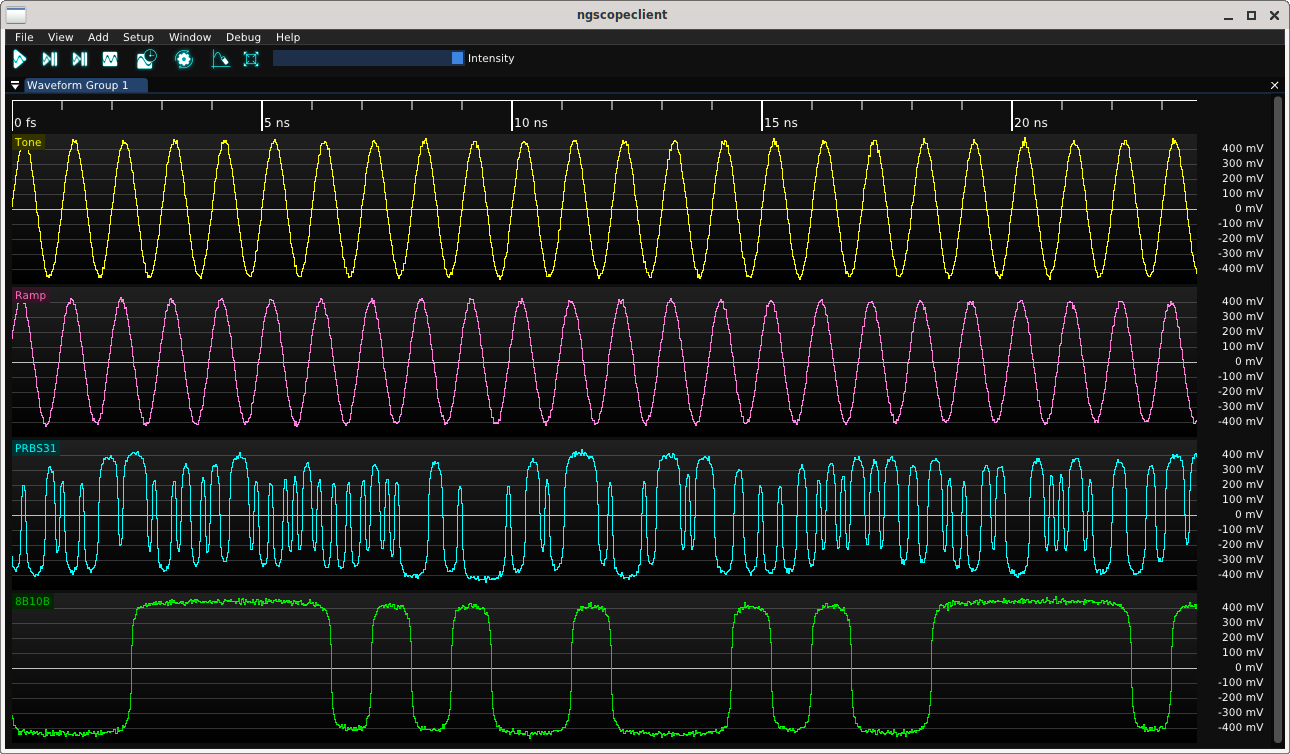
\includegraphics[width=13cm]{ng-images/overview.png}
\caption{Top level ngscopeclient window with a single waveform group}
\label{single-group}
\end{figure}

As you add protocol decodes or look at different parts of a waveform, it may be helpful to create additional waveform
groups. Typical reasons for creating additional groups include:

\begin{itemize}
\item Zooming into one set of signals to see detail on short time scales while maintaining a high level overview of
others
\item Viewing signals with incompatible horizontal units. For example, a FFT has horizontal units of frequency while an
analog waveform has horizontal units of time. Eye patterns also have horizontal units of time, but are always displayed
as two UIs wide and cannot be zoomed.
\end{itemize}

\section{Managing Groups}

New waveform groups are automatically created when adding a channel which is not compatible with any existing group.
For example, if your session has a single group containing time-domain waveforms, adding a FFT filter block will result
in a new waveform group being created to contain the FFT. Additional frequency-domain waveforms will then be added to
this group by default.

A new group may also be created at any time by clicking on a channel name and dragging it to the top, bottom, left, or
right edge of an existing group. An overlay (Fig. \ref{split-overlays}) will be displayed showing the resulting split.
For example, dropping the channel on the right side of the window produces the layout shown in Fig. \ref{split-right}.

\begin{figure}[h]
\centering
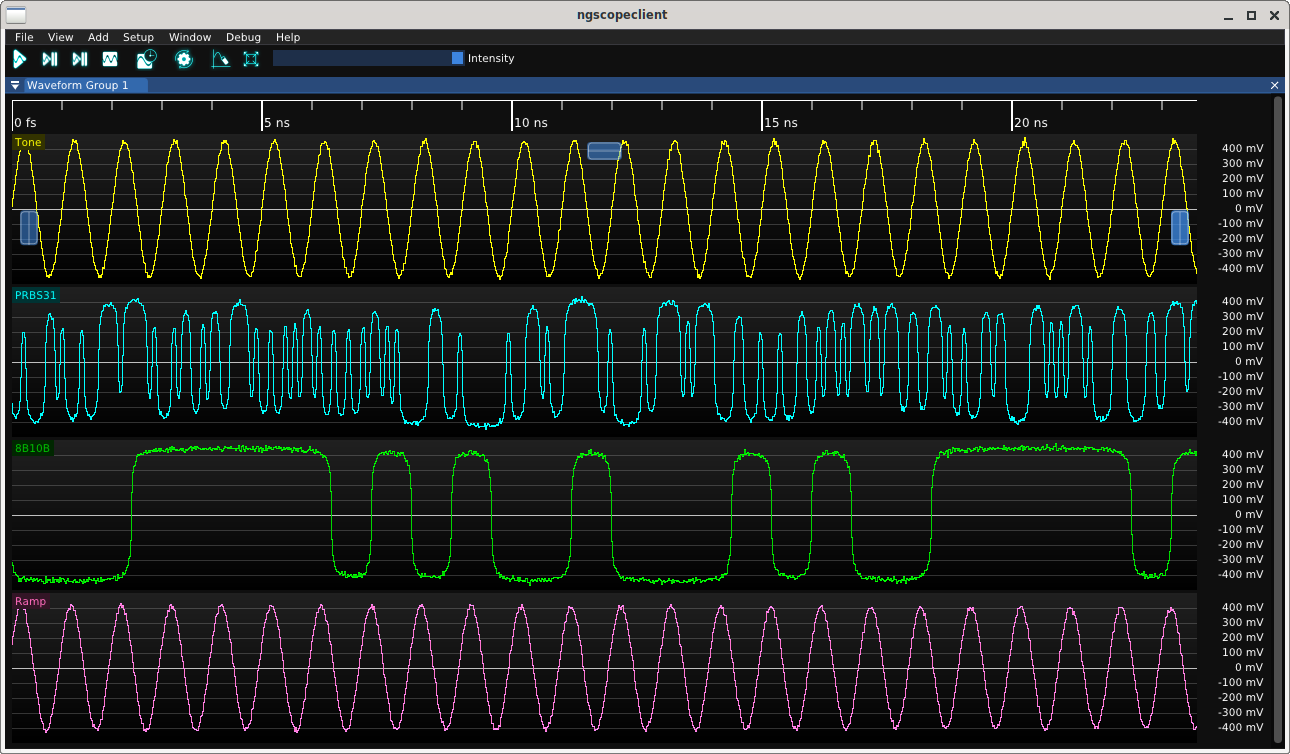
\includegraphics[width=13cm]{ng-images/split-overlays.png}
\caption{Overlays showing drag-and-drop locations for splitting waveform groups}
\label{split-overlays}
\end{figure}

\begin{figure}[h]
\centering
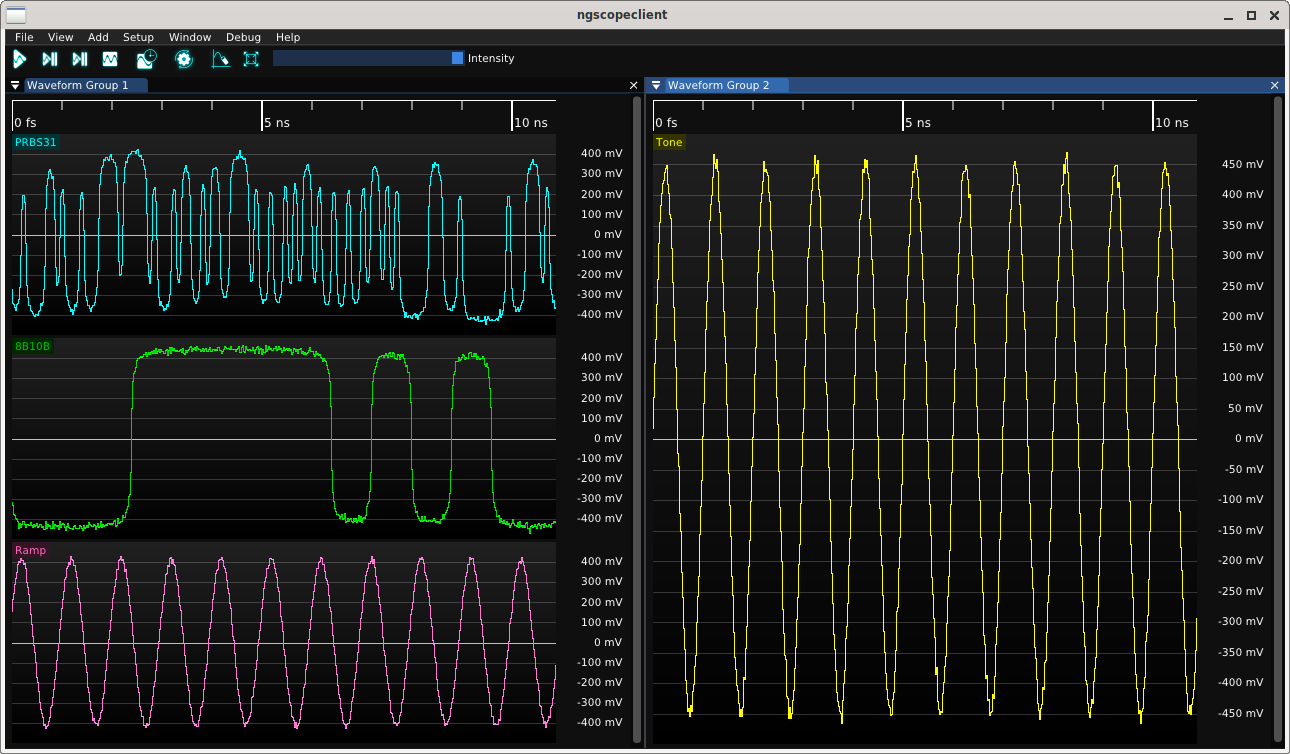
\includegraphics[width=13cm]{ng-images/split-right.png}
\caption{Result of dropping a waveform to the right side split area}
\label{split-right}
\end{figure}

Waveform groups may be resized arbitrarily by dragging the separator between them. The title bar of a group may also be
dragged, allowing the entire group to be undocked as a floating window. Floating windows can be re-docked by dragging
the title bar back into the main ngscopeclient window (or another floating window), creating new tabs or splitting
existing groups as desired (Fig. \ref{complex-ui}).

\begin{figure}[h]
\centering
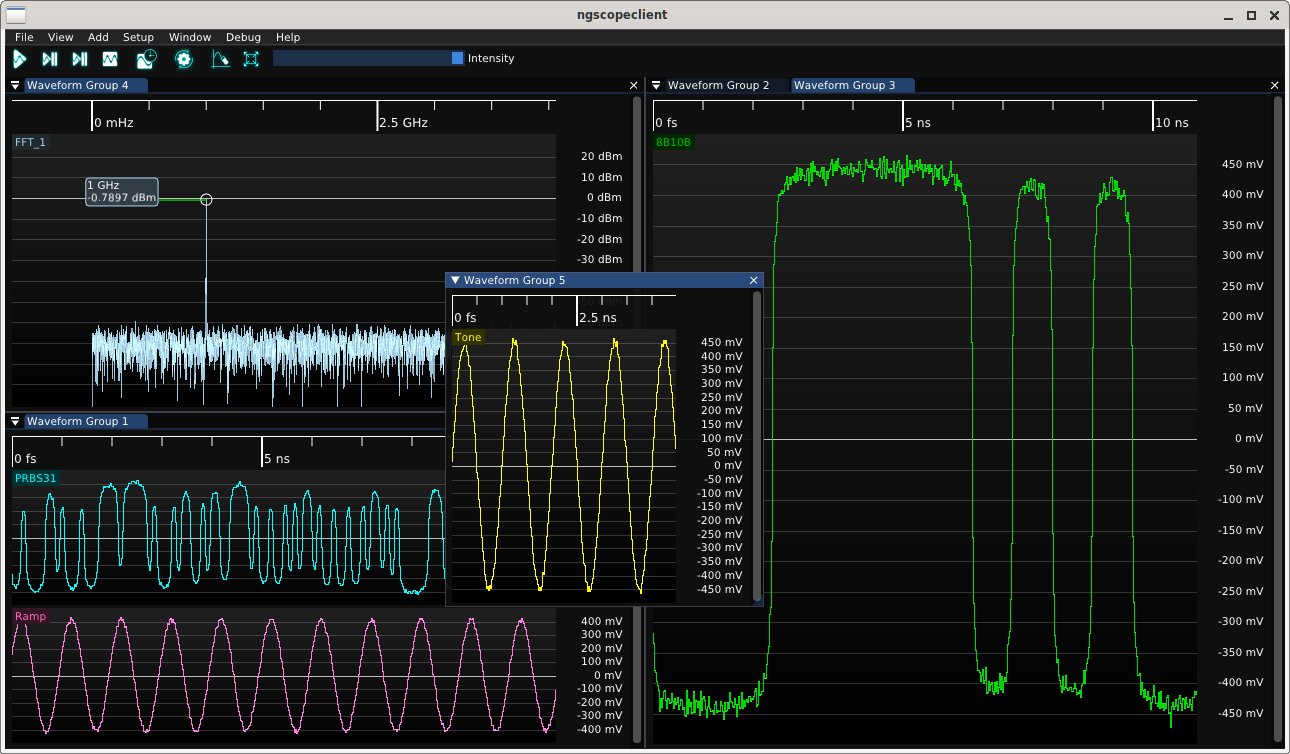
\includegraphics[width=13cm]{ng-images/complex-ui.png}
\caption{Example of complex window layout with multiple tabs, splitters between docked waveform groups, and a group in
a floating window}
\label{complex-ui}
\end{figure}
